\begin{frame}[fragile]{Файловая система. Данные и метаданные.}
    \begin{columns}
        \column{0.6\textwidth}
  \begin{block}{Упражнение. Выполнить команды. Расскажите что получили.}
    cat /etc/passwd
    \break
    stat /etc/passwd
  \end{block} 
        \column{0.3\textwidth}
        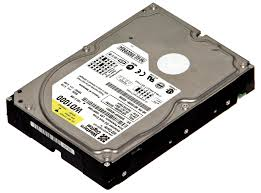
\includegraphics[height=3cm]{hw_hdd.jpg} 
    \end{columns}
\pause
Матаданные - информация о файле.
\begin{itemize}
 \item Размер файла
 \item Владелец и права доступа 
 \item Время доступа, изменения
\end{itemize}
\end{frame}
